\section{Source-To-Source Transformations}

This section describes the transformations that take Fortran elemental and
pure procedures as input and generate OpenCL kernels.

\subsection{OpenCL}

OpenCL~\cite{opencl:standard} is an open language standard for developing
applications for accelerators.  The C-based language provides extensions for
programming kernels that run on accelerator processing elements.  The kernels
are run by calling a C runtime library from the OpenCL host (normally the
CPU).  Efforts to standardize a C++ runtime are underway and Fortran
interfaces to the C runtime are described later.

An important concept in OpenCL is that of a thread and a thread group.  Thread
groups are used to run an OpenCL kernel concurrently on several processor
elements on the OpenCL device (often a GPU).  Consider a data-parallel
statement written in terms of an elemental fuction as discussed above.  The
act of running an OpenCL kernel can be thought of as having a particular
thread assigned to each instance of the call to the elemental function as it
is mapped across the arrays in the data-parallel statement.  In practice,
these threads are packaged into thread groups when they are run on the device
hardware.

Device memory is separated hierarchically.  A thread instance has access to
its own memory, thread groups to OpenCL local memory, and all thread groups
have access to OpenCL global memory.  When multiple members of a thread group
access the same memory elements, for example if {\tt region} or {\tt shift}
functions are called, for performance reasons it is often best if global
memory accessed by a thread group is copied into local memory.

The \emph{region} and \emph{halo} constructs easily map onto the OpenCL memory
hierarchy.  A schematic of this mapping is shown in Figure~\ref{fig:cl-memory}
for a two-dimensional array with a 2x2 array of 4 thread groups.  The memory
for the array and its halo are stored in global memory on the device as shown
in the background layer of the figure.  The array copy in local memory is
shown in the foreground divided into 4 \emph{local} tiles that partition the
array.  Halo regions in global memory are shown in dark gray and halo regions
in local memory are shown in light gray.

\begin{figure}[!t]
\centering
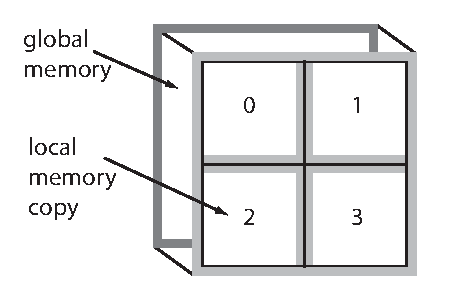
\includegraphics[width=2.5in]{cl-memory.pdf}
\caption{A schematic of global memory for an array and its copy stored in local memory
for four thread groups.}
\label{fig:cl-memory}
\end{figure}

We emphasize that the hierarchical distribution of memory used on the OpenCL
device shown in Figure~\ref{fig:cl-memory} can be extended to include memory
across MPI nodes as well.  In this case, the virtual global array is
represented by the background layer (with its halo) and its partitions stored
in the 4 MPI nodes shown in the foreground.

Halo regions are constrained semantically so that they can not be written to
by an OpenCL kernel because the \emph{region} and \emph{interior} functions
return copies of the global memory.  Thus once memory for a halo region has
been transferred into global device memory by all of the host nodes running
MPI (before the OpenCL kernel is run), memory is in a consistent state so that
the kernels are free to read from global device memory.  Because the local
memory is a copy, it functions as a software cache for the local thread group.
Thus the compiler must insert OpenCL barriers at proper locations in the code
to insure that all threads have written to the local memory cache before any
thread can read from the cache.  On exit from a kernel, the local memory cache
is copied back to global memory for all \emph{interior} regions leaving global
memory in a consistent state again.

\subsection{ForOpenCL}

This work describes transformations that automatically create OpenCL kernel
functions from Fortran pure and elemental procedures.  These transformations
will not transform an entire program.  Users, for now, must explicitly replace
calls to Fortran kernel procedures that run on the device, with calls to the
OpenCL runtime that will run the kernel on the OpenCL host.  While these host
transformations are straightforward using ROSE, they are outside the scope of
this paper.

In addition to the Fortran to OpenCL transformations, the
ForOpenCL~\cite{http:ofp} library provides programmers with the ability to
call the C OpenCL runtime from Fortran.  ForOpenCL is a set of Fortran modules
providing Fortran 2003 interface descriptions and classes that allow language
interoperability with the OpenCL runtime.


\section{Transformation examples}

This sections outlines the OpenCL equivalent syntax for portions of the
Fortran shallow-water code described in the previous section.  The notation
uses uppercase for arrays and lowercase for scalar quantities.  Interior and
region array copies are denoted by an i or an r preceeding the array.  For
example, {\tt iH = interior(H, halo)} is a local copy of interior region of
array {\tt H} (representing height) in the shallow water code.

\subsubsection{interior and region functions}

While the serial versions of the interior and regions functions return an
array copy, in OpenCL, these functions return a scalar quantity based on the
location of a thread in a thread group and the relationship of its location to
the array copy in local memory.  Because we assume there is a thread for every
element in the interior, the array index is just the thread index adjusted for
the halo.  Thus {\tt interior} and {\tt region} are just inline OpenCL
functions provided by the ForOpenCL library.

\subsubsection{function and variable declarations}

Fortran kernel procedures have direct correspondence with OpenCL equivalents.
For example, {\tt wave\_advance} is transformed as {\tt \_\_kernel void
  wave\_advance(\_\_ global float * H, ..., float dt);}.  The global state
variables have local equivalents, e.g., {\tt \_\_local float
  H\_local[MAX\_LOCAL\_SIZE]}, declared with the appropriate size and are copied
to local memory by the compiler with inlined library functions.  The flux
array temporaries (region variables) are declared similarly but initialized to
zero with inlined library functions.  Interior variables are simple scalars,
e.g., {\tt float iH;}.  Region variables cannot be scalar objects because
regions are shifted and thus \emph{shared} by threads within a thread group.

\subsubsection{array syntax}

Array syntax transforms nearly directly to OpenCL code.  For example, interior
variables are particularly straightforward as they as scalar quantities in
OpenCL,

{\small
\begin{verbatim}
iH = iH + (dt/dx) * (region(Ux, face_lt) - 
                     region(Ux, face_rt) )
        + (dt/dy) * (region(Vy, face_dn) - 
                     region(Vy, face_up) );
\end{verbatim}
}

Region variables are more complicated because they are arrays.

{\small
\begin{verbatim}
Hx[l] = 0.5 * (region(H_local, face_lt)+ ...);
\end{verbatim}
}

where {\tt l = LX + LY*(NLX+halo(0)+halo(1)))} is a local index variable, {\tt
  LX = get\_local\_id(0)} is the local thread id in the $x$ dimension, {\tt LY =
  get\_local\_id(1)} is the local thread id in the $y$ dimension, {\tt NLX =
  get\_local\_size(0)} is the size of the thread group in the $x$ dimension, and
the {\tt get\_local\_id} and {\tt get\_local\_size} functions are defined by the
OpenCL compiler.


\subsection{Performance measurements}

Performance measurements were made comparing the transformed code with
different versions of the serial shallow-water code.  The serial versions
include the original written in C and two Fortran versions: one using copy
semantics for the regions and one using reference semantics.  We also compare
with a hand written OpenCL implementation that was optimized for local memory
usage (no array temporaries).  The measurments were made using an NVIDIA Tesla C2050
GPU (TODO - need model numbers) running at XXX Hz and an Intel XXX hexacore CPU
running at XXX Hz with 2.56 GB of RAM.  The compilers were gfortran and gcc VERSIONS with
optimization of -O3.

The performance comparison is shown in Figure~\ref{fig:cl-performance} for
varying array sizes (of the state variables).  The time represents an average
of 100 iterations of the outer time-advance loop calling the OpenCL kernel.
This tight loop keeps the OpenCL kernel supplied with threads to take
advantage of potential latency hiding by the NVIDIA GPU.  Any serial code
within this loop would reduce the measured values.

As can be seen in Figure~\ref{fig:cl-performance}, the transformed get very
good results of roughly 65 times speedup over the best Fortran code and YYY
speedup over the original C code.  It comes with XXX \% of the hand coded
OpenCL version.

%\begin{figure}[!t]
%\centering
%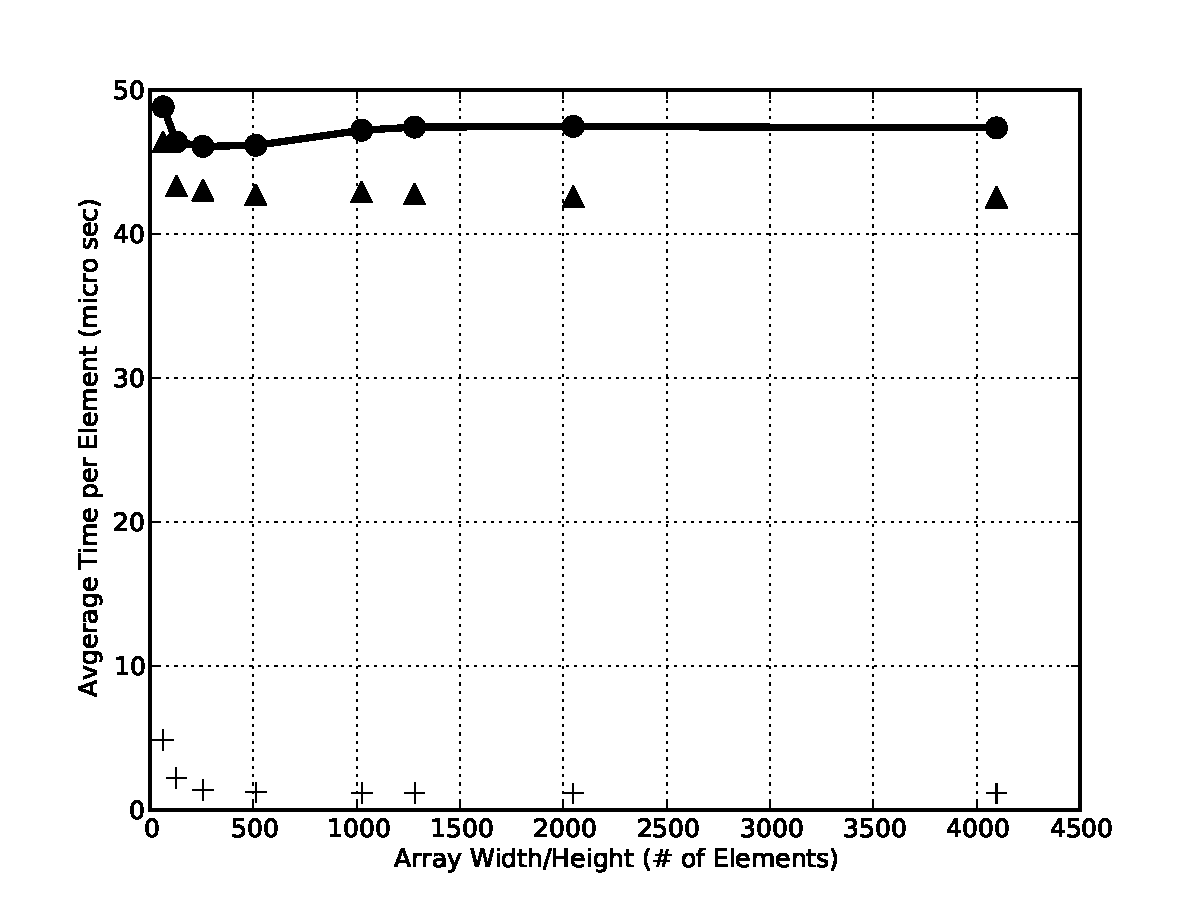
\includegraphics[width=2.5in]{cl-performance.pdf}
%\caption{Performance comparison for varying array size.}
%\label{fig:cl-performance}
%\end{figure}
